%!TEX root = info-main.tex
\section{Selfish Configuration in Wi-Fi Tethering}
\label{sec:channel-selection}

%%\subsection{Impact of Selfish Configuration in Wi-Fi Tethering}

To understand the impact of the selfish behavior of a Wi-Fi
tethering system using CCA tuning, we performed extensive simulations
with different transport-layer protocols (i.e., TCP and UDP,
in multi-AP environments) using the ns-2 simulator~\cite{NS2}.

%
\begin{figure} [t]
\center
  \subfigure[Topology-1]{  \label{fig-stopo1}
      \resizebox{26mm}{!}{
      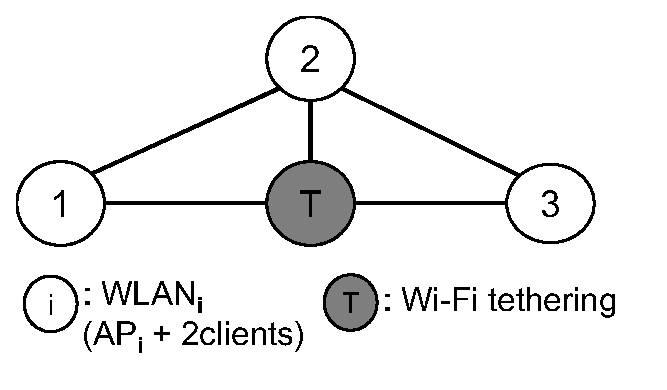
\includegraphics[]{./figures/FIG_sim_topo1}}
      }
  \subfigure[Topology-2]{ \label{fig-stopo2}
      \resizebox{30mm}{!}{
       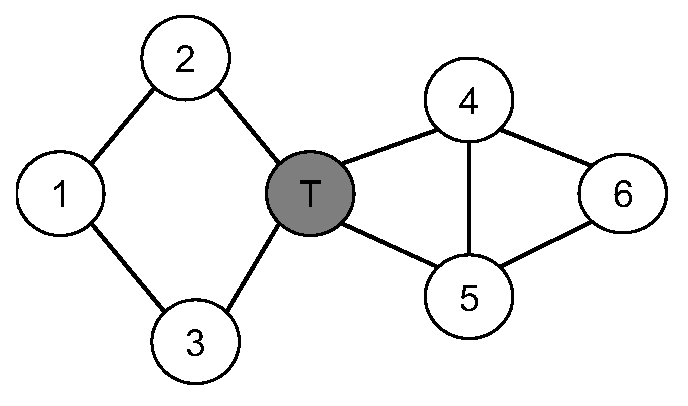
\includegraphics[]{./figures/FIG_sim_topo2}}
       }
    \caption{AP Interference graph of two simulated topologies.}
    \label{fig:sim_topology1}
\end{figure}
%
%
\begin{figure} [t]
  \subfigure[Topology-1, UDP]{  \label{fig-motive-udp-s1}
      \resizebox{40mm}{!}{
      \includegraphics[]{./figures/sim-motive-udp-M1}}
      }
  \subfigure[Topology-1, TCP]{ \label{fig-motive-tcp-s1}
      \resizebox{40mm}{!}{
       \includegraphics[]{./figures/sim-motive-tcp-M1}}
       }\\
       \subfigure[Topology-2, UDP]{  \label{fig-motive-udp-s2}
      \resizebox{40mm}{!}{
      \includegraphics[]{./figures/sim-motive-udp-M2}}
      }
  \subfigure[Topology-2, TCP]{ \label{fig-motive-tcp-s3}
      \resizebox{40mm}{!}{
      \includegraphics[]{./figures/sim-motive-tcp-M2}}
      }
\caption{Impact of selfish carrier sense on throughput of
transport-layer protocols over various cellular backhaul
link capacities $B_{cel}$ for tethering in two multi-AP topologies.}
    \label{fig:motive-ret1}
\end{figure}
%

\textbf{Multi-AP Topology}:
%
First, we study the impact when a selfish tethering launches within
a well-planned multi-AP network with two representative topologies.
%
The topologies used in the simulations are shown in
Fig.~\ref{fig:sim_topology1}.\footnote{We sampled the topologies from
a popular Wi-Fi database~\emph{Wigle}. For example, the topology shown
in Fig.~\ref{fig-stopo1} corresponds to the well-known FIM
(Flow-In-the-Middle) topology~\cite{FIM08}, which can be easily found
in real-world AP deployments~\cite{choi:shin12}. An edge in the
figure represents the neighboring interference, meaning that an AP is
in the carrier sensing range of its connected APs. The vertex denoted
by `T' in the figure represents the tethering system launched within
the network.}
%

We compare the performance for two cases using UDP and TCP protocols:
(i) \emph{Normal} scenario in which the \emph{host} node uses
the default CCA threshold, and (ii) \emph{Selfish} scenario in
which the \emph{host} node manipulates the MAC protocol by increasing
the CCA threshold as high as possible without losing the connectivity
to the guest.
%
We used the following settings in our simulations.
Each WLAN has an AP and two associated client nodes (i.e., 2 AP--clients
flows per WLAN), and all nodes operate on the same channel.
We considered typical IEEE 802.11a/g MAC/PHY parameters with the
maximum speed of 54\,Mbps, and set the capacity $B_{cel}$ of
the 3G/4G backhaul link of tethering to 5, 10, and 20\,Mbps.
Traffic is generated by a constant bit rate (CBR) traffic generator
for the UDP protocol (1\,KB packet size), and an FTP download
application is used to create TCP flows (1.5\,KB packet size).
% alex: the UDP traffic scenarios is not clear to me.
For UDP flows, we assume 10\,Mbps for flows in infrastructure APs,
and 20\,Mbps for tethering flows.


Fig.~\ref{fig:motive-ret1} shows the throughput of the tethering link
and APs. In \emph{Normal} case, we can see a throughput imbalance
among APs, and especially, the tethering flow is shown to experience
starvation due to the FIM problem~\cite{FIM08}.
%
With the CCA cheating, on the other hand, we can see that the
selfish tethering achieves a significant throughput gain at the cost
of significant throughput degradation for other nearby well-behaving
APs, for both UDP and TCP flows.
%
%Note that TCP is a bidirectional transfer-based protocol and
%here the CCA function is manipulated only on the host side,
%i.e., the \emph{guest} node is legitimate.
%
%Nevertheless, the selfish tethering achieves a high throughput gain
%with the TCP protocol.
%
Although we manipulate the CCA threshold only on the host side,
i.e., the \emph{guest} node is legitimate, the selfish tethering
achieves a high throughput gain even with the TCP protocol,
which is a bi-directional, transfer-based protocol.
%
This is attributed to the closed-loop TCP-ACK mechanism, i.e., the
more data packets (or ACKs) the legitimate guest successfully receives
from the misconfigured host, the more outstanding uplink ACKs (or data
packets) the guest can transmit.
%
% alex: what would be the toughput impact if we manipulate the CCA
% threshold from the guest node, more or less throughput gain?
The figure shows that the throughput gain increases proportional to
the cellular backhaul link bandwidth, $B_{cel}$, for both UDP and TCP
flows.


One can expect that selfish CCA manipulation would increase the
collision probability of the tethering link since the \emph{host}
node initiates packet transmission even in the present of other
nodes' transmissions. Nevertheless, we observe a significant gain
of selfish behavior using CCA manipulation, as seen from the above results.
%
To understand why the selfish tethering link can achieve a significant
gain with CCA manipulation, we investigate the property of the
successful receptions at the tethering receiver node, i.e.,
\emph{guest} node.
%
Table~II plots the collision probability, and the percentage of
successful receptions at the receiver in the simulation
with $B_{cell}$=10\,Mbps corresponding to the results shown
in Figs.~\ref{fig-motive-udp-s1} and \ref{fig-motive-udp-s2}, respectively.
We observe that, despite the high collision ratios (71.5\,\% and 91.8\,\%
for Topology 1 and 2, respectively), the tethered receiver can capture
the signal of interest (SoI), thanks to PHY capture effect and MIM.
A majority of the successful receptions are due to MIM, i.e., 63.6\,\%
and 63.5\,\% for Topology 1 and 2, respectively.
Note that the link distances between \emph{host} and \emph{guest}
nodes are very short, making the received signal at the \emph{guest}
node sufficiently stronger than the sum of interferences.

\begin{table}[ht]\label{table:ratio}
\renewcommand{\arraystretch}{1.2}
\caption{Statistics of receptions at the receiver (in case of UDP
and $B_{cell}$=10\,Mbps}
\vspace{-0.2cm}
\centering
\begin{tabular}{|c|c c c |}
\hline \bfseries Topology & Collision prob. & Capture effect & MIM\\
\hline\hline
1 & 71.5 & 17.9 & 63.6 \\
\hline
2 & 91.8 & 28.3 & 63.5 \\
\hline
\end{tabular}\label{tbl:txdist}
\end{table}

These results clearly demonstrate that the selfish behavior using CCA
manipulation abuses the short link distance property of Wi-Fi
tethering and thus makes it possible to exploit the benefits of MIM.
Consequently, the selfish tethering can achieve an unfair throughput
gain regardless of the network condition surrounding the tethering.

\begin{figure} [t]
\center
  \subfigure[Scenario 1]{  \label{fig-patialCH_a}
      \resizebox{24mm}{!}{
      \includegraphics[trim=0.0cm 0.25cm 0.0cm 0.0cm]{./figures/FIG_motive_topo_1a}}
      }
  \subfigure[Scenario 2]{ \label{fig-patialCH_b}
      \resizebox{31mm}{!}{
       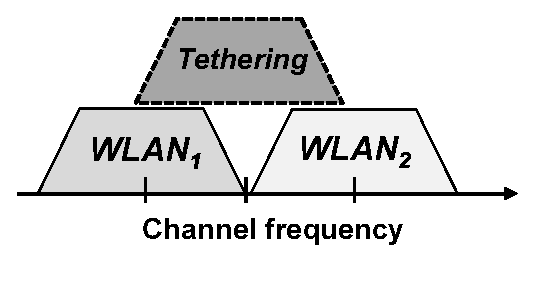
\includegraphics[trim=0.0cm 0.25cm 0.0cm 0.0cm]{./figures/FIG_motive_topo_1b}}
       }\\
  \subfigure[Throughput for Scenario 1]{  \label{fig-ret_patialCH_a}
      \resizebox{40mm}{!}{
      \includegraphics[trim=0.0cm 0.25cm 0.0cm 0.0cm]{./figures/FIG_sim-motiveA_24M}}
      }
  \subfigure[Throughput for Scenario 2]{ \label{fig-ret_patialCH_b}
      \resizebox{40mm}{!}{
       \includegraphics[trim=0.0cm 0.25cm 0.0cm 0.0cm]{./figures/FIG_sim-motiveB_24M}}
       }
    \caption{Impact of launching tethering on a partial-overlapped channel.}
    \label{fig:motive_A}
\end{figure}


%
\textbf{Impact of Tethering Channel}:
%
Next, we study the impact of the CCA manipulation on performance
when tethering is launched on a channel partially overlapping
with nearby APs. As mentioned above,
the tethered Wi-Fi hotspot can potentially set up the network with
an \emph{arbitrary} channel number, which may cause serious interference
to nearby well-planned APs.
We used two simple scenarios in \cite{zhang:shin11icnp} and the
channel model presented in \cite{Mishra:Arbaugh05} for our simulation.
Fig.~\ref{fig-patialCH_a} illustrates a simple case that the channel
selected by the tethering is partially overlapping with a nearby AP.
Since two overlapping channels are sensed by each other by the CCA
mechanism of 802.11, its effective spectrum usage is
only 20\,MHz \cite{zhang:shin11icnp}.
%
Fig.~\ref{fig-patialCH_b} depicts the case when the tethering shares
the spectrum with two adjacent orthogonal channels.
Note that in this case, the tethering link may suffer from channel
starvation \cite{zhang:shin11icnp}; the tethering link can transmit
only when both $WLAN_1$ and $WLAN_2$ are idle, but the probability of
the two outer channels being idle at the same time is very low
because the channel activities on the two outer channels are
asynchronous and may overlap randomly.

To evaluate the impact of the selfish behavior using CCA manipulation
in these scenarios, we performed simulations with following setting.
Each WLAN consists of two client nodes where the traffic on each flow
is generated with 10\,Mbps downlink CBR over UDP.
The capacity $B_{cel}$ for tethering is configured to 20\,Mbps
(with 20\,Mbps CBR/UDP traffic).
Initially, the tethering link is set to be legitimate.
The CCA manipulation is activated at 20\,s.

Figs.~\ref{fig-ret_patialCH_a} and \ref{fig-ret_patialCH_b} plot
the resulting throughput showing the effect of selfish behavior
using CCA manipulation.
When the tethering is legitimate, it achieves a fair share of shared
medium with two flows in $WLAN_1$ in the first scenario.
In the second case shown in Fig.~\ref{fig-patialCH_b},
the tethering is almost starved due to the channel starvation
problem \cite{zhang:shin11icnp}.
After the CCA value is configured selfishly,
despite the same unfair channel condition,
the tethering link achieves a significant throughput gain
at the cost of significant reduction in throughput of other flows.

In the same scenario depicted in Fig.~\ref{fig-patialCH_b},
we also compare the impact of CCA manipulation with
different types of selfish behavior manipulating other MAC parameters,
in particular manipulation of the backff mechanism using
smaller values of $CW_{min}$.\footnote{The manipulation of backoff mechanism
is widely adopted by selfish users~\cite{K:Vaidya05}.}
%
Fig.~\ref{fig:cwmin_cheat} shows the simulation results
with different values of $CW_{min}=$31,\,15,\,7,\,and 3.
%
The figure indicates that the selfish behavior using CCA manipulation
achieves throughput gain above those with smaller values of $CW_{min}$
and even higher than very aggressive setting with $CW_{min}=3$.
%
The results imply that the manipulation of CCA threshold is a simple,
yet more attractive approach that can be abused by adversaries in
a tethering environment.

\begin{figure} [ht]
\center
  \subfigure[2~client~nodes~per~WLAN]{ \label{fig-udp-10AP}
      \resizebox{33mm}{!}{
       \includegraphics[trim=0.5cm 0.25cm 0.5cm 0.25cm]{./figures/sim-comp_cw_N2}}
       }
       \subfigure[5~client~nodes~per~WLAN]{  \label{fig-tcp-10AP_downlink}
      \resizebox{33mm}{!}{
      \includegraphics[trim=0.5cm 0.25cm 0.5cm 0.25cm]{./figures/sim-comp_cw_N5}}
      }
    \caption{Throughput comparison with selfish configurations of the $CW_{min}$ parameter.}
    \label{fig:cwmin_cheat}
\end{figure}


%
\textbf{Impact of Cellular Backhaul Link Capacity}:
%
Finally, we evaluate the impact of the backhaul link capacity of
selfish tethering.
%
\begin{figure} [ht]
 \center{
        \scalebox{0.55}{\includegraphics{./figures/sim-sel-gain}}
       }
    \caption{Throughput gain of selfish carrier sensing over
various cellular backhaul link capacities and AP densities.}
    \label{fig:throughput-gain}
\end{figure}
%
Fig.~\ref{fig:throughput-gain} shows the throughput gain of the selfish
behavior as a function of backhaul link capacity for TCP and UDP
downlink traffic in a network with a high density of APs consisting
of 10 APs and 30 client nodes.
The figure indicates that the throughput gain is proportional to the
backhaul link capacity of the maximum achievable goodput determined
by the transport-layer protocol.\footnote{Note that in our simulation
when the backhaul apacity is larger than 20\,Mbps, the maximum
throughput is bounded by the Wi-Fi link capacity in this simulation.}
This is because the higher backhaul link capacity the tethering is
connected to, the more outstanding packets the selfish node can transmit.

%%
%% we will not include the following subsection this time
%%
\comment {%%%%%%%%%%%%%%%%%%%%%%%%%%%%%%%%%%%%%%%%%%%%%%%%%%
%
%
%
% COMMENT..

\subsection{Best Strategy of Selfish Tethering Nodes}

  %      [MIM Capture Effect]

For an adversary, the best selfish strategy is to increase the CCA
threshold as much as possible in order to increase his own throughput.


 %%  TODO: 아래 문구 수정. as much as possible
We now analytically show that, in tethering environments where
the link distance between host and guest devices is adjustable, a
selfish node can gain exclusive channel access while guaranteeing
a target frame reception ratio.
%
To derive the best strategy for the selfish node, we first need to
compute the throughput capacity of the tethered link.

Let $\theta_{s}$ denote the CCA threshold of node $s$ above which
node $s$ can correctly sense the symbols, and thus does not transmit
and freezes its backoff process \cite{ieee:80211-07}.
%
For given node $s$, we define the carrier sense set $C_{s}( \theta_{s} )$
as
%
\begin{equation} \label{eq:set_c}
C_{s} (\theta_s)= \{ k | G_{k, s} P_{0} > \theta_{s} \}.
\end{equation}
%
The nominal CCA threshold adopted by all legitimate nodes in the network
is denoted by $\theta_{0}$. By definition, for $\theta_s\!\geq\!\theta_{0}$,
$C_{s} (\theta_s) \! \subset C_{s}( \theta_0 )$.

From Eqs.~\eqref{eq:pathloss} and \eqref{eq:set_c},
the carrier sensing range, denoted by $R_{cs}$, is determined by the
CCA threshold, as:
\begin{equation}
R_{cs}(\theta) \! = \Big(\frac{ P_0 }{\theta} \Big)^{1/\alpha}.
\end{equation}

We consider 802.11g/n PHY which employs multiple modulation and
multiple coding schemes (MCSs) \cite{IEEE802.11n},
where the MCS schemes are listed in Table~I. %%%
%
%
Let $\gamma_{m}$ denote the minimum SIR requirement
(i.e., SIR threshold) for the successful reception at a receiver node
for each MCS scheme $m$.
%
Hence, for a transmission of node $s$ at MCS scheme $m$,
let $I_{r,m}$ be the \emph{interference set}  of nodes whose
simultaneous transmission will prevent node $r$ from correctly
decoding the frame from $s$:
\begin{equation}
I_{r, m} = \{ k | G_{k, r} P_{0} > \frac{ P_r }{ \gamma_{m} } \}.
\end{equation}

Hence, for a given MCS $m$, an interference occurs at receiver $r$ if
any node in $I_{r,m}$ transmits data simultaneously with transmitter $s$.

From the perspective of the sending node of an 802.11 link $i$
whose transmitter and receiver are denoted by $s$ and $r$, respectively,
the link's activity can be characterized with the following
three different channel states \cite{Gao:06}:
(a) \emph{self channel} occupied by the node's own transmission,
(b) \emph{busy channel} due to the activity of other neighboring nodes,
and (c) \emph{idle channel} when the channel is not used by any node.
%
Let ${x}_i(\theta_s)$, ${y}_{i}(\theta_s)$, and ${z}_{i}(\theta_s)$
denote, respectively, the fraction of time link $i$ stays in these
three states.
%
These variables are determined by the PHY- and MAC-layer
behavior of nearby 802.11 links, including link $i$
and neighboring links, with CCA threshold $\theta$.

Let $p_i(\theta_s)$ be the conditional transmission error
probability\footnote{The probability of an error seen by
a packet being transmitted at the receiver.} of link $i$,
given that a transmission attempt is made, which can be expressed:
\begin{eqnarray}
p(\theta_s)=&P[\text{simultaneous TX in }C_{r}(\theta_s)]\!\cdot\
\!P[\text{not capture effect}] \nonumber \\
&+ P[\text{no TX in }C_{r}(\theta_s)]\!\cdot\
\!P[\text{TX in }I_{r}],
\end{eqnarray}
where $TX$ is an abbreviation for transmission.
%
Then, the available throughput capacity $S_i(\theta)$ of link $i$
with CCA threshold $\theta_s$ is given by
\begin{equation}
S_i(\theta_s) = {x}_i(\theta_s) \times \Big(1 - p_i(\theta_s)\Big) \times R_i \times
\frac{T_{payload}}{T_{tx}},
\end{equation}
where $R_i$ is the data transmission rate, $T_{payload}$ is the
average transmission time of the data payload, and
$T_{tx} = T_{Header} + T_{payload}+ SIFS + (Block)ACK + DIFS $
is the average overall transmission time (in number of time slots) for
a packet, including PHY and MAC headers, data payload and ACK, as well
as DCF Inter-frame Space (DIFS) and Shortest Inter-frame Space (SIFS).
Since we are only interested in the \emph{maximum} available
capacity of link $i$, we assume that the node always has
backlogged packets to transmit.

In 802.11 MAC, nodes attempt to transmit only during an idle slot.
In other words, the sender node counts down its backoff timer
to transmit a packet only during idle periods, and it defers the
count-down process whenever the channel is sensed busy.
Thus, if we let $\tau(p)$ model the attempt rate per idle slot for
a given transmission-error probability $p$ \cite{Kumar:07Fixed},
then the normalized self airtime ${X}_i(c)$ is proportional to
the normalized idle-time ${Z}_i(c)$ and can be expressed as:
\begin{equation}
{x}_i(\theta) = {z}_i(\theta) \times \tau\big(p_i(\theta)\big) \times T_{tx}.
\end{equation}
%
Therefore, we obtain the throughput capacity $S_i(\theta)$ of link $i$
on channel $c$ as
\begin{equation}\label{eq:linkcapacity}
S_i(\theta) =  {z}_i(\theta) \times \tau\big(p_i(\theta)\big) \times \Big(1 - p_i(\theta)\Big)
\times R_i \times T_{payload}.
\end{equation}
%
Note that the data rate $R_i$ is determined by the
physical link condition of link $i$.
%%---1

Based on the above equation showing the relation between the throughput
of a link ad its CCA threshold $\theta$, we have the following proposition.

\begin{proposition}[Proposition 1]
When the link distance is less than a certain value, by manipulating
the CCA threshold, a selfish node can gain exclusive channel access
without reducing the frame reception ratio.
\end{proposition}
%\vspace{0.15cm}
\begin{proof}
%%
%%
See Appendix A.
\end{proof}
%%

Thus, an adversary user can  gain exclusive channel access in
tethering environments where the link distance between the host and
guest devices is controllable to gain an unfair advantage in
throughput performance by manipulating the tethering function.
For example, by rooting or jailbreaking mobile OSes, the channel
access functions of Wi-Fi protocol can be manipulated ``selfishly,''
at the cost of other nearby well-behaving Wi-Fi devices' performance.
Therefore, detecting unauthorized and misconfigured tethering Wi-Fi
is becoming a very important task in most organizations.

} %%%% COMMENT
